\label{capitolo4}
\section{Tecnology Mapping}
Il tecnology mapping � una fase di ottimizzazione che si colloca sotto l'ottimizzazione tecnology indipendent. Questa operazione consiste nell'assegnare alle diverse funzioni logiche del circuito una serie di porte in base a delle librerie che contengono una serie di porte. Queste librerie vengono chiamate \emph{cell library}.
Esistono due approcci per effettuare il tecnology mapping il primo � abbastanza euristico basato su regole di sostituzione di tipo tecnology indipendent molto efficente per piccoli circuiti ma richiede un tempo eccessivo di computazione.\\
Il secondo approccio invece si basa su algoritmi; si divide in diversi passi primo dei quali � trasformare la rete attraverso una serie di funzioni base. Il grafo cos� formato viene detto \emph{subject graph} tipicamente formato solo da porte NAND a due ingressi e da inverter. Il secondo passo dell'algoritmo � rappresentare anche le funzioni di libreria mediante l'utilizzo di porte NAND e inverter, questo genera il cosidetto \emph{pattern graphs}
\begin{figure}[hb]
\centering
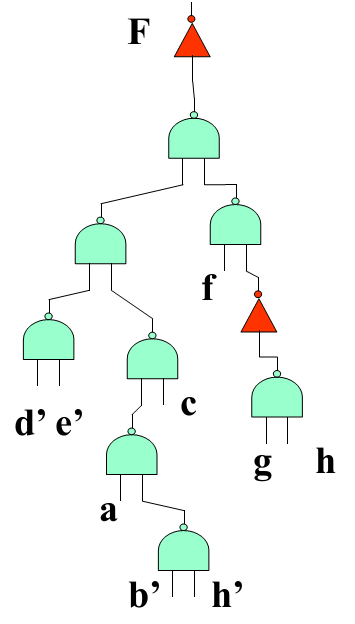
\includegraphics[height=9cm]{img/subject.png}
\caption{Esempio di subject graph}
\label{fig:subject}
\end{figure}
\subsection{algoritmo}
Terminata la fase di preparazione si passa alla fase in pi� propriamente algoritmica. Lo scopo � quello di effettuare la miglior \emph{copertura} del grafo, ovvero, fare in modo che ogni nodo del subject graph sia contentuto in uno o pi� pattern graph. inoltre ogni input di un pattern graph deve essere l'output di qualche altro grafo.\\
I diversi algoritmi devono trovare la copertura di costo minimo migliore per il subject graph sottoposto all'analisi.
\begin{figure}[thb]
\centering
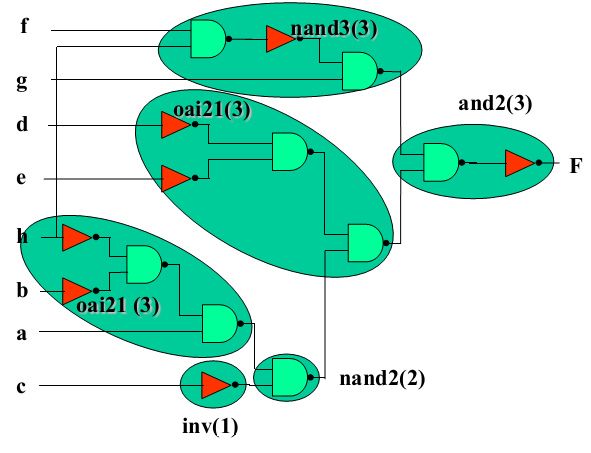
\includegraphics[width=10cm]{img/copertura.png}
\caption{Esempio di copertura con porte AND OR-AND a 2+1 ingressi e NAND a 3 ingressi}
\label{fig:copertura}
\end{figure}
\subsection{Copertura DAG}
Il tecnology mapping utilizzando il metodo DAG richiiede come ingresso la rete ottimizzata e descritta in modo indipendente dalla tecnologia e la libreria di porte da utilizzare. Esso restituisce la netlist di porte che minimizza il costo totale.\\
Il meccanismo � quello di verificare tutte le possibili combinazioni \{$m_k$\} per ogni nodo e impostando ($m_i=1$) tutte le variabili per il quale il pattern graph � scelto. Dopodiche si scrivono una serie di clausule per ogni nodo del subject graph indicando quali match sono stati effettuati. Ripetendo tale operazione per tutti i nodi e moltiplicando le varie clausule si ottiene la soluzione cercata
\begin{table}[hbt]
\centering
\begin{tabular}{c|c|c|c|c|}
&$m_1$&$m_2$&\dots&$m_k$\\
\hline
$n_1$&&&&\\
\hline
$n_2$&&&&\\
\hline
$\vdots$&&&&\\
\hline
$n_l$&&&&\\
\hline
\end{tabular}
\caption{Esempio di tabella di copertura}
\label{tab:t_copertura}
\end{table}
\subsection{Optimal tree covering}
Nel caso particolare in cui la nostra rete logica sia ad albero, ovvero non vi � la presenza di fanout esiste un algoritmo pi� efficente per trovare la copertura migliore.\\
Il principo � quello di coprire gli alberi in modo ottimale usando la programmazione dinamica. L'assunzione che si fa � che per ogni figlio dell'albero si conosce in modo ricorsivo il costo migliore per la copertura e si assume che gli ingressi abbiano costo 0. A questo punto il costo totale � dato dalla somma di tutti i costi.
\begin{verbatim}
Algorithm OPTIMAL_AREA_COVER(node) {
	foreach input of node {
		OPTIMAL_AREA_COVER(input);// satisfies recurs. assumption
	}
	// Using these, find the best cover at node 
	node->area = INFINITY;
	node->match = 0;
	foreach match at node {
		area = match->area;
		foreach pin of match {
			area = area + pin->area;
		}
		if (area < node->area) {
			node->owarea = area;
			node->match = match;
		}
	}
}
\end{verbatim}

